\documentclass{cornouaille}
\dscornouaille
\begin{document}
\cornouaille{TS}{Eval 7 - 1 heure}{Vendredi 14 février 2020}

\begin{definiton}[Une définition]

un truc la

\end{definiton}

\Bareme
\begin{exercice}[Les bases][1.5]
	Simplifier les expressions suivantes:
	\begin{multicols}{3}
	$A=\frac{3-\ln(\text{e})}{\ln(9)}$\\
	\ldotcarreaux[5]
	
		$B=\frac{\ln(\text{e})}{\ln(e^2)}+ \ln\left(\frac{1}{e}\right)$\\
	\ldotcarreaux[5]
	
			$C=\frac{\ln(6)-\ln(12)}{2\ln(\sqrt{2})}$\\
	\ldotcarreaux[5]
	\end{multicols}
\end{exercice}
%%%%%%%%%%%%%%%%%%%%%%%%%%%
\begin{exercice}[Equations-Inéquations][6]
Résoudre :
\begin{enumerate}
	\item $2\ln(x)=\ln(2-x)$\\
	\ldotcarreaux[7]
	\item $2(\ln(x))^2+\ln(x)-1=0$\\
	\ldotcarreaux[7]
	\item $\ln(1-2x)-\ln(2)\leq \ln(x+1)+\ln(3)$\\
	\ldotcarreaux[7]
	\item Déterminer le plus petit entier $n$ tel que $0,85^n\leq 0,05$\\
	\ldotcarreaux[7]
\end{enumerate}	
\end{exercice}
%%%%%%%%%%%%%%%%%%%%%%%%%%%
\begin{exercice}[Dérivation][2.5]
	Déterminer les fonctions dérivées des fonctions suivantes sur leur ensemble de définition:
	\begin{enumerate}
		\item $f(x)=x+2\ln(x+2)$ sur $D_f=]-2;+\infty[$\\
	\ldotcarreaux[6]
		%\item $g(x)=\frac{\ln(x)}{x+1} $ sur $D_g=]0;+\infty[$\\
	%\ldotcarreaux[5]
		\item $h(x)=3(\ln(x))^2+2\ln(x)$ sur $D_h=]0;+\infty[$\\
	\ldotcarreaux[6]
	\end{enumerate}
\end{exercice}
%%%%%%%%%%%%%%%%%%%%%%%%%%%
\begin{exercice}[Limites][5]
	Déterminer les limites suivantes:
	\begin{enumerate}
		\item $\Lim{x}{+\infty}{\ln(2+3e^x)}$\\
	\ldotcarreaux[6]
		\item $\Lim{x}{0^+}{\ln(2+3e^x)}$\\
	\ldotcarreaux[6]
		\item $\Lim{x}{+\infty}{(\ln(x))^2-3\ln(x)}$\\
	\ldotcarreaux[6]
			\item $\Lim{x}{0^+}{(\ln(x))^2-3\ln(x)}$\\
	\ldotcarreaux[6]
	\end{enumerate}
\end{exercice}
\newpage 
%%%%%%%%%%%%%%%%%%%%%%%%%%%
\begin{exercice}[Logarithmes][7]
On considère la fonction $f$ définie sur $]O;+\infty[$ par: $f(x) = \ln(x)-2x^2$
\begin{enumerate}
	\item \'Etudier les variations de $f$.\\
	\ldotcarreaux[5]
\setbar{2}
\begin{solution}
$f'(x)=\frac{1}{x}-4x=\frac{1-4x^2}{x}$

Comme $x \in ]0;+\infty[$, $f'(x)$ est du signe de $1-4x^2=(1-2x)(1+2x)$.

Après le tableau de signes (à faire !),\\
\begin{tikzpicture}
	\tkzTabInit{$x$ / 0.85 , $1-4x^2$ / 0.5 }
	{$-\infty$ , $-\frac{1}{2}$, $\frac{1}{2}$ , $+\infty$}
	\tkzTabLine{,-,z,+,z,-,}
\end{tikzpicture} \\
on en déduit que $f$ est strictement croissante sur $]0;\frac{1}{2}[$ et strictement décroissante sur $]\frac{1}{2};+\infty[$.
\end{solution}
	\item Déterminer les limites de $f$ en 0 et en $+\infty$. Que peut-on en déduire ?\\
	\ldotcarreaux[6]
\setbar{2}
\begin{solution}
Aucune difficulté en 0. On trouve: $\lim_{x\to 0}f(x)=-\infty$.

On peut en déduire que l'axe des ordonnées est asymptote verticale à la courbe.

En $+\infty$:

$f(x)=\ln(x) - 2x^2 = x\left(\frac{\ln(x)}{x} -2x\right)$ et on utilise $\lim_{x\to +\infty} \frac{\ln(x)}{x} =0$.

On trouve $\lim_{x\to +\infty}f(x)=-\infty$
\end{solution}
	\item Dresser le tableau de variations de $f$.\\
	\ldotcarreaux[3]
	
\setbar{0.5}
\begin{solution}
\begin{tikzpicture}
	\tkzTabInit{$x$ / 0.85 , $f'(x)$ / 0.5 , $f(x)$ / 1.5}
	{$0$ , $\frac{1}{2}$, $+\infty$}
	\tkzTabLine{,+,z,-,}
	\tkzTabVar{-/ $-\infty$, +/ $\ln\left(\frac{1}{2}\right)-\frac{1}{2}$ , -/ $-\infty$  }
\end{tikzpicture}
\end{solution}
	\item Quel est le signe de $f$ sur $]0;+\infty[$ ? Justifier.\\
	\ldotcarreaux[2]
\setbar{1}
\begin{solution}
Le maximum sur $]0;+\infty[$ est $\ln\left(\frac{1}{2}\right)-\frac{1}{2} \approx -1,2$ 
on en déduit : $\forall x \in ]0;+\infty[ : f(x) <0$ 
\end{solution}
	\item Démontrer que l'équation $f(x)=-2$ admet exactement deux solution $\alpha$ et $\beta$ sur $]0;+\infty[$. En donner une valeur approchée arrondie à $10^{-3}$ près.\\
	\ldotcarreaux[6]
\setbar{1.5}
\begin{solution}
\begin{itemize}
	\item Sur l'intervalle $\left] 0; \frac{1}{2}\right ]$ la fonction $f$ est continue (car dérivable) et est strictement croissante à valeurs dans $\left]-\infty;\ln\left(\frac{1}{2}\right)-\frac{1}{2} \right]$ \\
	$-2 \in \left]-\infty; \ln(\frac{1}{2})-\frac{1}{2} \right]$ , alors d'après le corolaire du théorème des valeurs intermédiaires : l'équation $f(x)=-2$ admet une unique solution $\alpha$ sur $\left]0;\frac{1}{2} \right]$ .\\
	On a de plus $0,1408 <\alpha <0,1409 $ donc $\alpha \approx 0,141$ à $10^{-3}$ près 
	\item Sur l'intervalle $\left] \frac{1}{2}; +\infty \right[ $ la fonction $f$ est continue (car dérivable) et est strictement décroissante à valeurs dans $\left]-\infty; \ln(\frac{1}{2})-\frac{1}{2} \right]$ \\
	$-2 \in \left]-\infty; \ln(\frac{1}{2})-\frac{1}{2} \right]$  , alors d'après le corolaire du théorème des valeurs intermédiaires : l'équation $f(x)=-2$ admet une unique solution $\beta$ sur  $\left] \frac{1}{2}; +\infty \right[ $ . \\
	On a de plus $\beta =1$
\end{itemize}
\end{solution}
\end{enumerate}
\end{exercice}
%%%%%%%%%%%%%%%%%%%%%%%%%%%
\end{document}